\section{METODOLOGIA EXPERIMENTAL}


\subsection{Materiais}

\begin{itemize}
\item Foi utilizado o simulador Simulink do Matlab para simular os seguintes experimentos.
\end{itemize}


\subsection{M�todos}
Na primeira atividade, foi montado o circuito da figura abaixo com ajuda do roteiro que continha todos os par�metros necess�rios para configurar os blocos:

\begin{figure}[H]
    \centering
    \caption{Sistema PAM retangular com filtro.}
    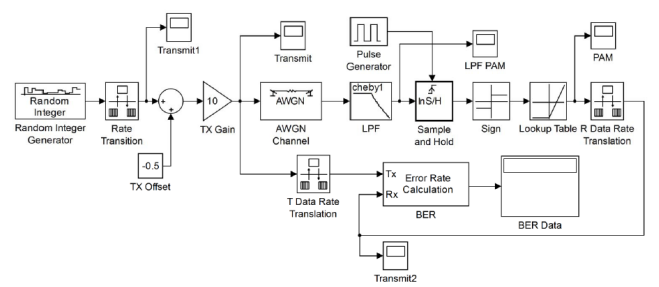
\includegraphics[scale=0.8]{Imagens/f1}
    \label{f1}
\end{figure}

 
Os par�metros de simula��o foram feitos assim: start time 0; stop time 10.001; type: fixed-step; solver: ode3; fixed-step size 2e-5; period sample time constraint: unconstrained; tasking mode for period sample times: auto.

Ap�s isto, encontramos os dados obtidos em cada osciloscopio, simulado no circuito : transmit 1, transmit, transmit 2, LPF PAM e PAM.

Deveriamos tamb�m verificar o atraso no sinal recebido em rela��o ao sinal transmitido.

E para finalizar este exercicio, deveriamos plotar o gr�fico BER X SNR, utilizando a fun��o semilogy e preencher uma tabela. * Obs. Considerando a pot�ncia do sinal de 25W. 

\begin{center}
    \begin{table}[H]
        \caption{Taxa de erro de bit.}
        \centering\begin{tabular}{c|c|c}
            SNR[dB] & AWGN $\sigma^2$ & BER \\ \hline
            0.96  & 20 &  \\
            & 50 & 0,0001 \\
            & 100 &  \\
            & 150 &   \\
            & 200 &   \\
            & 250 &  \\
            & 270 &  \\
            & 300 &  \\
            & 500 &  \\ \hline
        \end{tabular}
    \end{table}
\end{center}

Na segunda atividade, deveriamos simular o circuito PAM sinc que estende-se al�m de um tempo de bit, mas evita a interfer�ncia intersimb�lica (ISI) pelo fato de ter valores zeros em $\pm nTb$ (n � um inteiro e $n \neq 0$).

E todos os par�metros foram configurados de acordo com o roteiro.

\begin{figure}[H]
    \centering
    \caption{PAM com sync.}
    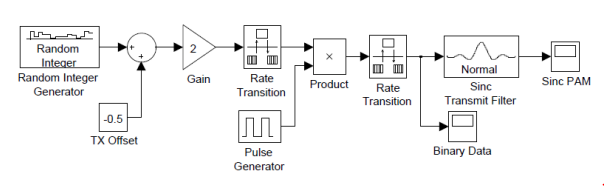
\includegraphics[scale=1]{Imagens/f2}
    \label{f2}
\end{figure}

Depois de simulado o circuito deveriamos obter os gr�ficos obtidos nos oscilosc�pios para uma taxa de bit de   e  . 

Em seguida deveriamos obter como terceira atividade a densidade espectral de pot�ncia do      PAM sinc e para isto, os blocos do circuito foram reconfigurado de acordo com o roteiro e a simula��o foi feita utilizando os seguintes param�tros.

start time 0; stop time 10; type: fixed-step; solver: ode3; fixed-step size 2e-5; period sample time constraint: unconstrained; tasking mode for period sample times: auto.

Por conseguinte, deveriamos gerar o gr�fico dos espectros de pot�ncia  do sinal,observando os pontos de zero, que se encontram no eixo x.


E como ultima atividade do laborat�rio, tivemos que simular um circuito para verificar o desempenho do PAM sinc em um receptor simples AWGN.

\begin{figure}[H]
    \centering
    \caption{Sistema PAM sync.}
    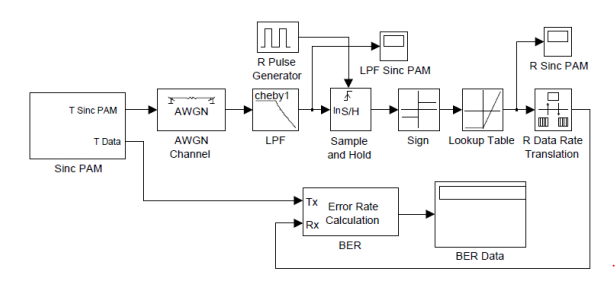
\includegraphics[scale=1]{Imagens/f3}
    \label{f3}
\end{figure}

Os par�metros de simula��o foram os seguintes:

Ao final da simula��o deveriamos obter os gr�ficos gerados pelos oscilosc�pios presentes no circuito.

Tamb�m tinhamos que obter o atraso no sinal recebido com rela��o ao sinal enviado e ainda plotar o gr�fico BER x SNR e preencher a tabela abaixo:

Sabendo que a pot�ncia do sinal � de aproximadamente 24,3 W era necess�rio calcular a pot�ncia do sinal.

\begin{figure}[H]
    \centering
    \caption{Calculo do valor RMS.}
    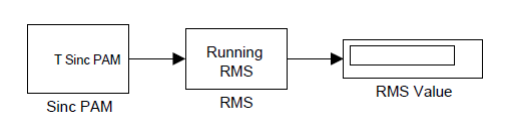
\includegraphics[scale=0.8]{Imagens/f4}
    \label{f4}
\end{figure}


\begin{center}
    \begin{table}[H]
        \caption{Taxa de erro de bit.}
        \centering\begin{tabular}{c|c|c}
            SNR[dB] & AWGN $\sigma^2$ & BER \\ \hline
             0.85  & 20 &  \\
              & 50 & 0,0001 \\
              & 100 &  \\
              & 150 &   \\
             & 200 &   \\
             & 250 &  \\
             & 270 &  \\
             & 300 &  \\
             & 500 &  \\ \hline
        \end{tabular}
    \end{table}
\end{center}

\newpage
